

%!TEX root=../protocol.tex	% Optional

\section{Einführung}
Für die IT-Abteilung der Höheren Technischen Bundeslehranstalt TGM soll für
Lernbüroklassen ein neues Anwesenheitskontroll-Konzept umgesetzt werden.
Lernbüroschüler können selbst ihren Unterricht auswählen und einteilen, um
einen selbstbestimmteren Schulablauf zu ermöglichen. Um die dazugehörige
Bürokratie in Bezug auf Anwesenheit zu verringern, sollen Kartenleser
installiert werden, um die Anwesenheitskontrolle automatisiert abwickeln zu
können.
\begin{comment}
\section{Zielbestimmung}
Bis zum 20.12.2018 soll die Entwicklung eines Kartenlesers als Muster für die Lernbüroklassen abgeschlossen sein. Auf diesem sollen Schüler ihre Schülerkarte einlesen, um sich im Lernbüro anmelden und identifizieren zu können. Der Kartenleser soll die eingelesenen Daten dann an den \gls{zps} weiterleiten, welcher diese dann verarbeitet und in die \gls{lba} einträgt.\\
Durch die Installation solcher Kartenleser kann der Anmeldevorgang deutlich schneller und reibungsloser gestaltet werden. Außerdem werden automatisch Datensätze
zur Anwesenheit der Schüler generiert und müssen nicht mehr händisch aus den
Klassenbüchern abgetippt werden, was die dafür benötigte Bearbeitungszeit entfallen lässt und somit Lehrkräfte entlastet.
\end{comment}
\section{Voruntersuchung}
\subsection{Ist-Zustand}
Derzeit wird für die Anwesenheitskontrolle der Lernbüroklassen auf Klassenbücher zurückgegriffen. In diese werden die Anwesenheiten vorerst händisch von der Lehrkraft eingetragen und dann später in die \gls{lba} übertragen. Diese beinhaltet eine Datenbank welche die Anwesenheiten speichert und den einzelnen Stundenblöcken zuordnet. Da dieser Prozess aufwändig und eher umständlich ist, soll auf ein neues auf Kartenleser-gestütztes System umgestiegen werden.

\subsection{Alternativen}
Die heutzutage für Firmen üblichen Anmeldesysteme, welche Kartenleser und dergleichen implementieren, wären für eine Schule viel zu komplex und nicht auf den Schulablauf zugeschnitten. Deshalb wird ein einfacheres, individuell angepasstes System gesucht, welches im Funktionsumfang schlanker und in der Anschaffung auch preiswerter ist. Für den \gls{zps} gibt es auch kein Alternativsystem, da die Software an das in der Schule bereits installierte System angepasst werden muss. 
\section{Produktauswahl}
\subsection{Trendanalyse}
Digitale Klassenbücher erlangen immer mehr Beliebtheit. Einige Schulen haben den Schritt weg vom Papier bereits geschafft und viele weitere werden folgen. Auch das \glqq freie Lernen'' erlangt immer mehr Aufmerksamkeit in der Bevölkerung. 
\subsection{Marktanalyse}
Zurzeit gibt es kein Produkt, welches die Anwesenheitskontrolle von Schulklassen erleichtert. Mit dem \gls{lbvt} kommt das erste Produkt seiner Art auf den Markt. Dadurch ist der Markt komplett offen und alle Schulen mit einem digitalen Klassenbuch können als potentielle Kunden angesehen werden. Auch der Umstieg auf ein digitales Klassenbuch wird somit vereinfacht, weshalb Schulen die einen Umstieg erwägen ebenfalls unsere Kunden sein könnten.
\section{Soll-Zustand}
\subsection{Muss-Ziele}
\begin{coloritemize}
    \item \textbf{\textcolor{gray}{Schülerkarten einlesen}}  \\ 
        Es soll ein mobiler Kartenleser erstellt werden, der Schülerkarten einlesen kann und die damit verbundenen Anmeldedaten an einen \gls{zps} senden kann. 
    
    \item \textbf{\textcolor{gray}{Kartenleser-Datensicherung implementieren}}  \\ 
        Falls der \gls{zps} aus verschiedensten Gründen nicht erreichbar ist und die Anmeldedaten vom Kartenleser nicht empfangen kann, müssen diese lokal am Kartenleser gesichert werden. 
        
    \item \textbf{\textcolor{gray}{\gls{zps} realisieren}}  \\
        Es soll ein Zwischenplattform-Server realisiert werden, der Anmeldedaten von Kartenlesern empfangen und verarbeiten kann. Der Server soll, mit Hilfe einer lokalen Datenbank, die Schüler-ID aus den empfangenen Anmeldedaten erfassen und einem Schüler zuordnen. Die Verarbeiteten Daten sollen an eine Schnittstelle der \gls{lba} übertragen werden, um dort die Anwesenheit der Schüler grafisch darstellen zu können.
        
    \item \textbf{\textcolor{gray}{Grafische Oberfläche für Kartenleserverwaltung erstellen}}  \\ 
        In der \gls{lba} soll eine Unterseite für Kartenleser erstellt werden, wo authentifizierte Personen die Systemdaten des Kartenlesers abrufen können. Weiters kann dem Kartenlesern ein Raum zugeordnet werden.
        
    \item \textbf{\textcolor{gray}{Daten verschlüsseln}}  \\
        Die Daten, die zwischen Kartenleser und \gls{zps} gesendet werden, sollen verschlüsselt sein. Das Verschlüsselungsverfahren soll gut zwischen Performance und Sicherheit ausbalanciert sein.
        
    \item \textbf{\textcolor{gray}{Hardware erweitern}}  \\
        Die zur Reproduktion der Hardware des \gls{lbvt} benötigten Schritte werden in Form eines Handbuches abgelegt. Außerdem wird dem Kunden ein \gls{speicherabbild} vom Kartenleser-Muster übergeben, um leichter neue Kartenleser aufzusetzen.
    
\end{coloritemize}
\newpage

\subsection{Kann-Ziele}
\begin{coloritemize}
    \item \textbf{\textcolor{gray}{Alle Klassen mit Kartenlesern ausstatten}}  \\
        Das Projektteam soll alle Klassen der Abteilung IT mit Kartenlesern ausstatten. Weiters sollen diese konfiguriert werden und dem lokalen \gls{zps} zugewiesen werden.
        
    \item \textbf{\textcolor{gray}{Voranmeldungssoftware erstellen}}  \\    
        Das \gls{lbvt} soll um eine Voranmeldungssoftware erweitert werden. In dieser sollen sich Lernbüroschüler zeitlich vor den Unterrichtseinheiten für einen Gegenstand eintragen können. Die Voranmeldungssoftware soll in die \gls{lba} eingebettet werden.  
\end{coloritemize}
%\subsection{Nicht-Ziele}

\newpage
\section{Produktfunktionen}
\subsection{Kartenleser Funktionen}
\begin{itemize}[leftmargin=1.0in]
    % Kartenleser-Funktionen
    \item [\lf] Karten einlesen \\
        Die Schüler sollen ihre Schülerkarte beim Kartenleser einlesen können. Das Einlesen soll durch eine drahtlose Kommunikation zwischen Kartenleser und Schülerkarte erfolgen.
\end{itemize}
\begin{flushright}
    \begin{tabular}{| A{3cm}  A{6.5cm} | c | c |}
        \hline \rowcolor{gray} \textbf{\textcolor{white}{Funktion}} && \textbf{\textcolor{white}{Nutzen}} & \textbf{\textcolor{white}{Aufwand}}\\
        \hline \hline
        Name & \lflast Karten einlesen & Hoch & Mittel \\
        Kurzbeschreibung & Schüler liest Schülerkarte am Kartenleser ein, um Anwesenheit zu bestätigen &&  \\
        Auslöser & Schüler liest seine Karte am Kartenleser ein &&  \\
        Ergebnis & Die Schüler-ID wurde vom Kartenleser eingelesen &&  \\
        Akteure & Schüler und Kartenleser &&  \\
        Eingehende $   $Information & Einlesebefehl &&  \\
        Ausgehende  Information & Speicherungsbefehl &&  \\
        Vorbedingungen & Kartenleser muss eingeschaltet und funktionsfähig sein &&  \\
        Nachbedingungen & Vor erneutem Einlesen muss die Speicherung der vorherigen Einlesung abgeschlossen sein  &&  \\
        \hline
    \end{tabular}
\end{flushright}    
\newpage

\begin{itemize}[leftmargin=1.0in]      
    \item [\lf] Daten speichern \\
        Die durch die Funktion /LF0010/ eingelesenen Daten sollen im Speicher des Kartenlesers abgelegt werden. Dieser Speicher dient als Zwischenspeicher und Backupsystem, damit im Falle einer Störung, in der der \gls{zps} aus verschiedenen Gründen die Daten des Kartenlesers nicht annehmen kann, die Daten immer noch am Kartenleser gesichert sind und zu einem späteren Zeitpunkt wieder gesendet werden können. 
        % \\ Das erfolgreiche Speichern ruft die Funktion /LF0060/ aus.
\end{itemize}
\begin{flushright}
    \begin{tabular}{| A{3cm}  A{6.5cm} | c | c |}
        \hline \rowcolor{gray} \textbf{\textcolor{white}{Funktion}} && \textbf{\textcolor{white}{Nutzen}} & \textbf{\textcolor{white}{Aufwand}}\\
        \hline \hline
        Name & \lflast Daten speichern & Hoch & Mittel \\
        Kurzbeschreibung & Der Kartenleser speichert die eingelesene ID mit Beschreibungen als Anmeldedaten in seinem Zwischenspeicher ab &&  \\
        Auslöser & Schülerkarte wurde eingelesen &&  \\
        Ergebnis & Die eingelesenen Daten sind im Zwischenspeicher abgespeichert &&  \\
        Akteure & Kartenleser &&  \\
        Eingehende $   $Information & Speicherungsbefehl &&  \\
        Ausgehende  Information & Sendebefehl und Ausführung des Einlese-Feedbacks &&  \\
        Vorbedingungen & Kartenleser muss funktionsfähig sein und Zwischenspeicher darf nicht voll sein &&  \\
        Nachbedingungen & Die eingelesenen Daten sind im Zwischenspeicher abgelegt  &&  \\
        \hline
    \end{tabular}
\end{flushright}     
\newpage
        
\begin{itemize}[leftmargin=1.0in]  
    \item [\lf] Kartenleser-Daten senden \\
        Nach erfolgreichem Speichern, sollen die im Zwischenspeicher vorhandenen Daten an den \gls{zps} gesendet werden. 
\end{itemize}
\begin{flushright}
    \begin{tabular}{| A{3cm}  A{6.5cm} | c | c |}
        \hline \rowcolor{gray} \textbf{\textcolor{white}{Funktion}} && \textbf{\textcolor{white}{Nutzen}} & \textbf{\textcolor{white}{Aufwand}}\\
        \hline \hline
        Name & \lflast Kartenleser-Daten senden & Hoch & Hoch \\
        Kurzbeschreibung & Die im Zwischenspeicher abgelegten Anmeldedaten werden an das \gls{zps} gesendet &&  \\
        Auslöser & Die eingelesenen Anmeldedaten wurden im Zwischenspeicher abgelegt und sollen wieter gesendet werden &&  \\
        Ergebnis & Bei funktionierender Netzwerkverbindung wurden die Daten an das \gls{zps} gesendet  &&  \\
        Akteure & Kartenleser und \gls{zps} &&  \\
        Eingehende $   $Information & Sendebefehl &&  \\
        Ausgehende  Information & Netzwerk-Paket mit Anmeldedaten  &&  \\
        Vorbedingungen & Kartenleser muss funktionsfähig sein und die genutzte Netzwerkverbindung muss stabil sein &&  \\
        Nachbedingungen & Keine  &&  \\
        \hline
    \end{tabular}
\end{flushright} 
\newpage

\begin{itemize}[leftmargin=1.0in] 
    \item [\lf] \gls{zps}-Daten empfangen \\
        Um eine Rückmeldung vom \gls{zps} empfangen zu können, muss der Kartenleser Daten vom diesem empfangen können. 
\end{itemize}
\begin{flushright}
    \begin{tabular}{| A{3cm}  A{6.5cm} | c | c |}
        \hline \rowcolor{gray} \textbf{\textcolor{white}{Funktion}} && \textbf{\textcolor{white}{Nutzen}} & \textbf{\textcolor{white}{Aufwand}}\\
        \hline \hline
        Name & \lflast \gls{zps}-Daten empfangen & Hoch & Hoch \\
        Kurzbeschreibung & Der Kartenleser empfängt Daten vom \gls{zps} &&  \\
        Auslöser & \gls{zps} hat Daten vom Kartenleser erfolgreich erhalten und will dies dem Kartenleser mit einem \gls{ack} berichten &&  \\
        Ergebnis & Der Kartenleser kann seine gesendeten Daten von seinem Zwischenspeicher löschen &&  \\
        Akteure & Kartenleser und \gls{zps} &&  \\
        Eingehende $   $Information & \gls{ack} &&  \\
        Ausgehende  Information & Löschungsbefehl &&  \\
        Vorbedingungen & Kartenleser muss funktionsfähig sein und die genutzte Netzwerkverbindung muss stabil sein &&  \\
        Nachbedingungen & Keine  &&  \\
        \hline
    \end{tabular}
\end{flushright} 
\newpage

\begin{itemize}[leftmargin=1.0in] 
    \item [\lf] Zwischenspeicher leeren \\
        Falls der Kartenleser eine positive Rückmeldung, ein sogenanntes \\ \gls{ack}, vom \gls{zps} bekommt,  %was bedeutet, dass die Schülerkarten-Daten erfolgreich an das Serversystem übermittelt wurden, 
        sollen alle Schülerdaten die übergeben wurden, vom Zwischenspeicher entfernt werden.
\end{itemize}
\begin{flushright}
    \begin{tabular}{| A{3cm}  A{6.5cm} | c | c |}
        \hline \rowcolor{gray} \textbf{\textcolor{white}{Funktion}} && \textbf{\textcolor{white}{Nutzen}} & \textbf{\textcolor{white}{Aufwand}}\\
        \hline \hline
        Name & \lflast Zwischenspeicher leeren & Hoch & Mittel \\
        Kurzbeschreibung & Erfolgreich gesendete Anmeldedaten werden vom Zwischenspeicher gelöscht &&  \\
        Auslöser & Der Kartenleser hat vom \gls{zps} ein \gls{ack} erhalten &&  \\
        Ergebnis & Die erfolgreich gesendeten Daten werden vom Zwischenspeicher gelöscht &&  \\
        Akteure & Kartenleser &&  \\
        Eingehende $   $Information & Löschungsbefehl &&  \\
        Ausgehende  Information & Keine &&  \\
        Vorbedingungen & Kartenleser muss funktionsfähig sein &&  \\
        Nachbedingungen & Gesendete Daten wurden vom Zwischenspeicher gelöscht  &&  \\
        \hline
    \end{tabular}
\end{flushright} 
\newpage

\begin{itemize}[leftmargin=1.0in] 
    \item [\lf] Einlese-Feedback \\
        Das erfolgreiche Einlese mit Speicherung einer Schülerkarte soll entweder ein auditives oder visuelles Feedback am Kartenleser zurückgeben.
\end{itemize}
\begin{flushright}
    \begin{tabular}{| A{3cm}  A{6.5cm} | c | c |}
        \hline \rowcolor{gray} \textbf{\textcolor{white}{Funktion}} && \textbf{\textcolor{white}{Nutzen}} & \textbf{\textcolor{white}{Aufwand}}\\
        \hline \hline
        Name & \lflast Einlese-Feedback & Hoch & Mittel \\
        Kurzbeschreibung & Erfolgreiches Einlesen und Speichern von Anmeldedaten erzeugt bzw. gibt ein auditives oder visuelles Feedback &&  \\
        Auslöser & Anmeldedaten wurden erfolgreich am Kartenleser gespeichert &&  \\
        Ergebnis & Ein auditives oder visuelles Einlese-Feedback wird angezeigt &&  \\
        Akteure & Kartenleser &&  \\
        Eingehende $   $Information & Feedbackbefehl &&  \\
        Ausgehende  Information & Positive sichtbare oder hörbare Ausgabe einer Ausgabeeinheit am Kartenleser &&  \\
        Vorbedingungen & Kartenleser muss funktionsfähig sein und mit einem Ausgabegerät bestückt sein &&  \\
        Nachbedingungen & Keine  &&  \\
        \hline
    \end{tabular}
\end{flushright} 
\newpage




    % Server-Funktionen
    \lfn
\subsection{\gls{zps} Funktionen}
\begin{itemize}[leftmargin=1.0in]
    %\item [\lf]  Anmeldedaten speichern\\
      %  Der Server speichert die Anmeldedaten der Schüler in einer Datenbank ab. Welche Daten gespeichert werden ist bei Produktdaten unter den  spezifiziert.\\
      % Unnötig da das ganze als unter den Produktdaten eh schon definiert ist. Wir brauchen keine extra fkt dafür
        
    %\item[\lf] Anmeldedaten empfangen und entschlüsseln\\
        %Der Kartenleser sendet gemäß /LD0050/ Daten an den Server. Dieser verfügt über eine Schnittstelle mit welcher er die Informationen empfangen kann. Die Daten werden vor der Weiterverarbeitung entschlüsselt.
    
    \item[\lf] Kartenleser-Daten empfangen\\
        Der Kartenleser sendet gemäß /LD0050/ Daten, die die Anmeldungen von Schülern per Karten-ID enthalten, an den \gls{zps}. Dieser verfügt über eine Schnittstelle, mit welcher er die Informationen empfangen kann. %Die Daten werden vor der Weiterverarbeitung entschlüsselt.
    
            \end{itemize}
\begin{flushright}
    \begin{tabular}{| A{3cm}  A{6.5cm} | c | c |}
        \hline \rowcolor{gray} \textbf{\textcolor{white}{Funktion}} && \textbf{\textcolor{white}{Nutzen}} & \textbf{\textcolor{white}{Aufwand}}\\
        \hline \hline
        Name & \lflast Kartenleser-Daten empfangen & Hoch & Mittel \\
        Kurzbeschreibung & Der \gls{zps} verfügt über eine Schnittstelle mit welcher er Daten vom Kartenleser empfängt &&  \\
        Auslöser & Kartenleser sendet Daten an den \gls{zps}&&  \\
        Ergebnis & \gls{zps} verarbeitet empfangene Daten weiter &&  \\
        Akteure & \gls{zps} und Kartenleser &&  \\
        Eingehende $   $Information & Daten vom Kartenleser gemäß /LD0050/ &&  \\
        Ausgehende  Information & Die Karten-ID des Schülers an /LF0120/ &&  \\
        Vorbedingungen & Kartenleser \& \gls{zps} sind miteinander Verbunden &&  \\
        Nachbedingungen & Keine  &&  \\
        \hline
    \end{tabular}
\end{flushright} 
\newpage
    \begin{itemize}[leftmargin=1.0in]
    
    
    \item[\lf] Daten verarbeiten und weitersenden\\
        Der \gls{zps} übersetzt die empfangene Karten-ID auf einen eindeutigen Schüler um. Anhand von den Daten des Kartenlesers wird dem Schüler automatisch die Anwesenheit für den Raum, in dem sich der Kartenleser befindet, eingetragen. Sobald alle benötigten Daten gesammelt wurden, werden diese an die \gls{lba} weitergesendet, damit hier ebenfalls die Anwesenheit eingetragen werden kann. Am Anfang des Prozesses wird überprüft, ob der Schüler bereits anwesend ist und gegebenenfalls wird die weitere Verarbeitung der Daten abgebrochen.
        
        \end{itemize}
\begin{flushright}
    \begin{tabular}{| A{3cm}  A{6.5cm} | c | c |}
        \hline \rowcolor{gray} \textbf{\textcolor{white}{Funktion}} && \textbf{\textcolor{white}{Nutzen}} & \textbf{\textcolor{white}{Aufwand}}\\
        \hline \hline
        Name & \lflast Daten verarbeiten und weitersenden & Hoch & Hoch \\
        Kurzbeschreibung & Der \gls{zps} übersetzt die empfangene Karten-ID auf einen eindeutigen Schüler und trägt dessen Anwesenheit ein &&  \\
        Auslöser & Daten wurden erfolgreich vom \gls{zps} empfangen &&  \\
        Ergebnis & Die Anwesenheit des Schülers wurde eingetragen &&  \\
        Akteure & \gls{zps} und \gls{lba} &&  \\
        Eingehende $   $Information & Karten-ID des Schülers &&  \\
        Ausgehende  Information & Ein \gls{ack}, siehe /LF0130/ &&  \\
        Vorbedingungen & Karten-ID muss einem Schüler zuordenbar sein &&  \\
        Nachbedingungen & Derselbe Schüler kann sich nicht für einen anderen Raum als anwesend eintragen  &&  \\
        \hline
    \end{tabular}
\end{flushright} 
\newpage
    \begin{itemize}[leftmargin=1.0in]
    \item[\lf] \gls{zps}-Daten senden \\ %Anmelde-Daten wurden erfolgreich Empfangen\\
        Der \gls{zps} sendet ein \gls{ack} an den Kartenleser, der die Daten gesendent hat, zurück, sobald gültige Anmelde-Daten empfangen und gespeichert wurden.
        % ka wie viel Sinn es hat Ack-packets zu verschlüsseln... notfalls borko/umar fragn
      
      
      
\end{itemize}
\begin{flushright}
    \begin{tabular}{| A{3cm}  A{6.5cm} | c | c |}
        \hline \rowcolor{gray} \textbf{\textcolor{white}{Funktion}} && \textbf{\textcolor{white}{Nutzen}} & \textbf{\textcolor{white}{Aufwand}}\\
        \hline \hline
        Name & \lflast \gls{zps}-Daten senden  & Hoch & Niedrig \\
        Kurzbeschreibung &  Bei erfolgreicher verarbeitung der Daten, welche der Kartenleser gesendet hat wird ein \gls{ack} zurückgeschickt&&  \\
        Auslöser & Daten wurden erfolgreich vom \gls{zps} verarbeitet &&  \\
        Ergebnis & Ein \gls{ack} wurde an den Kartenleser gesendet &&  \\
        Akteure & \gls{zps} und Kartenleser &&  \\
        Eingehende $  $Information & Daten welcher bereits verarbeitet wurden &&  \\
        Ausgehende  Information & Ein \gls{ack} an den Kartenleser &&  \\
        Vorbedingungen & \gls{zps} und Kartenleser sind miteinander verbunden  &&  \\
        Nachbedingungen & Keine  &&  \\
        \hline
    \end{tabular}
\end{flushright} 
\newpage 
       
\begin{itemize}[leftmargin=1.0in]

    \item[\lf] Klassenliste einlesen\\
        Der \gls{zps} kann Klassenlisten einlesen und diese in seiner lokalen Datenbank speichern.
        
        
\end{itemize}
\begin{flushright}
    \begin{tabular}{| A{3cm}  A{6.5cm} | c | c |}
        \hline \rowcolor{gray} \textbf{\textcolor{white}{Funktion}} && \textbf{\textcolor{white}{Nutzen}} & \textbf{\textcolor{white}{Aufwand}}\\
        \hline \hline
        Name & \lflast Klassenliste einlesen & Mittel & Hoch \\
        Kurzbeschreibung & Der \gls{zps} kann Klassenlisten einlesen &&  \\
        Auslöser & Eine autorisierte Person gibt dem \gls{zps} eine Klassenliste &&  \\
        Ergebnis & Die Klasssenliste wurde in einer Datenbank auf dem \gls{zps} gespeichert &&  \\
        Akteure & \gls{zps} und autorisierte Person &&  \\
        Eingehende $   $Information & Klassenliste &&  \\
        Ausgehende  Information & Ob das speichern der Klassenliste erfolgreich war &&  \\
        Vorbedingungen & Keine &&  \\
        Nachbedingungen & Keine  &&  \\
        \hline
    \end{tabular}
\end{flushright} 
\newpage

\lfn
\subsection{Funktionen für die Grafische Oberfläche in der \gls{lba}}
\begin{itemize}[leftmargin=1.0in]
    % GUI-Funktionen
    \item [\lf] Kartenleserdaten anzeigen \\
        Über die grafische Oberfläche in der \gls{lba} sollen die IDsder einzelnen Kartenleser mit ihren derzeitigen Räumen in einer Tabelle angezeigt werden können.
\end{itemize}
\begin{flushright}
    \begin{tabular}{| A{3cm}  A{6.5cm} | c | c |}
        \hline \rowcolor{gray} \textbf{\textcolor{white}{Funktion}} && \textbf{\textcolor{white}{Nutzen}} & \textbf{\textcolor{white}{Aufwand}}\\
        \hline \hline
        Name & /LF0210/ Kartenleserdaten anzeigen & Hoch & Mittel \\
        Kurzbeschreibung & Zeigt die ID des Kartenlesers in einer Tabelle gemeinsam mit dem Raum an &&  \\
        Auslöser & Autorisierte Lehrkraft öffnet grafische Oberfläche in der \gls{lba} &&  \\
        Ergebnis & Die ID des Kartenlesers wird neben dem Raum in einer Tabelle angezeigt &&  \\
        Akteure & Autorisierte Lehrkraft &&  \\
        Eingehende $   $Information & Aufruf der grafischen Oberfläche &&  \\
        Ausgehende  Information & Ausgabe der Daten in einer Tabelle &&  \\
        Vorbedingungen & Korrekter Aufruf der grafischen Oberfläche &&  \\
        Nachbedingungen & Keine  &&  \\
        \hline
    \end{tabular}
\end{flushright}
\newpage
\begin{itemize}[leftmargin=1.0in]
    % GUI-Funktionen
    \item [\lf] Raumzuteilung anzeigen \\
        Gemeinsam mit der ID des Kartenlesers sollen, in der grafischen Oberfläche der \gls{lba}, auch die derzeitig eingetragenen Räume zu den Kartenlesern angezeigt werden können.
\end{itemize}
\begin{flushright}
    \begin{tabular}{| A{3cm}  A{6.5cm} | c | c |}
        \hline \rowcolor{gray} \textbf{\textcolor{white}{Funktion}} && \textbf{\textcolor{white}{Nutzen}} & \textbf{\textcolor{white}{Aufwand}}\\
        \hline \hline
        Name & /LF0220/ Raumzuteilung anzeigen & Hoch & Mittel \\
        Kurzbeschreibung & Zeigt den Namen des Raumes in dem sich der Kartenleser befindet gemeinsam mit der ID des Kartenlesers in einer Tabelle an &&  \\
        Auslöser & Autorisierte Lehrkraft öffnet grafische Oberfläche in der \gls{lba} &&  \\
        Ergebnis & Der Name des Raumes wird neben der ID des jeweiligen Kartenlesers in einer Tabelle angezeigt &&  \\
        Akteure & Autorisierte Lehrkraft &&  \\
        Eingehende $   $Information & Aufruf der grafischen Oberfläche &&  \\
        Ausgehende  Information & Ausgabe der Daten in einer Tabelle &&  \\
        Vorbedingungen & Korrekter Aufruf der grafischen Oberfläche &&  \\
        Nachbedingungen & Keine  &&  \\
        \hline
    \end{tabular}
\end{flushright}
\newpage
\begin{itemize}[leftmargin=1.0in]
    \item [\lf] Kartenleser den Räumen zuordnen \\
        Über die grafische Oberfläche in der \gls{lba} soll außerdem die Möglichkeit bestehen den einzelnen Kartenleser Räume zuzuordnen. Diese Zuordnung soll dann im System gespeichert werden und den anderen Funktionen zu Verfügung stehen.
\end{itemize}
\begin{flushright}
    \begin{tabular}{| A{3cm}  A{6.5cm} | c | c |}
        \hline \rowcolor{gray} \textbf{\textcolor{white}{Funktion}} && \textbf{\textcolor{white}{Nutzen}} & \textbf{\textcolor{white}{Aufwand}}\\
        \hline \hline 
        Name & /LF0230/ Kartenleser den Räumen zuordnen & Hoch & Mittel \\
        Kurzbeschreibung & Die Raumzuteilung der Kartenleser kann geändert werden &&  \\
        Auslöser & Autorisierte Lehrkraft möchte Raumzuteilung ändern &&  \\
        Ergebnis & Der neue Raum ist in der Ansicht eingetragen und im System gespeichert &&  \\
        Akteure & Autorisierte Lehrkraft &&  \\
        Eingehende $   $Information & Änderungsanfrage mit neuem Raum des Kartenlesers&&  \\
        Ausgehende  Information & aktualisierte grafische Oberfläche in der \gls{lba} &&  \\
        Vorbedingungen & Ein korrekter Raum muss dem Kartenleser zugeteilt werden &&  \\
        Nachbedingungen & Der geänderte Raum ist im System gespeichert und steht den anderen Funktionen zu Verfügung &&  \\
        \hline
    \end{tabular}
\end{flushright}
\subsection{Aktivitätsdiagramm}
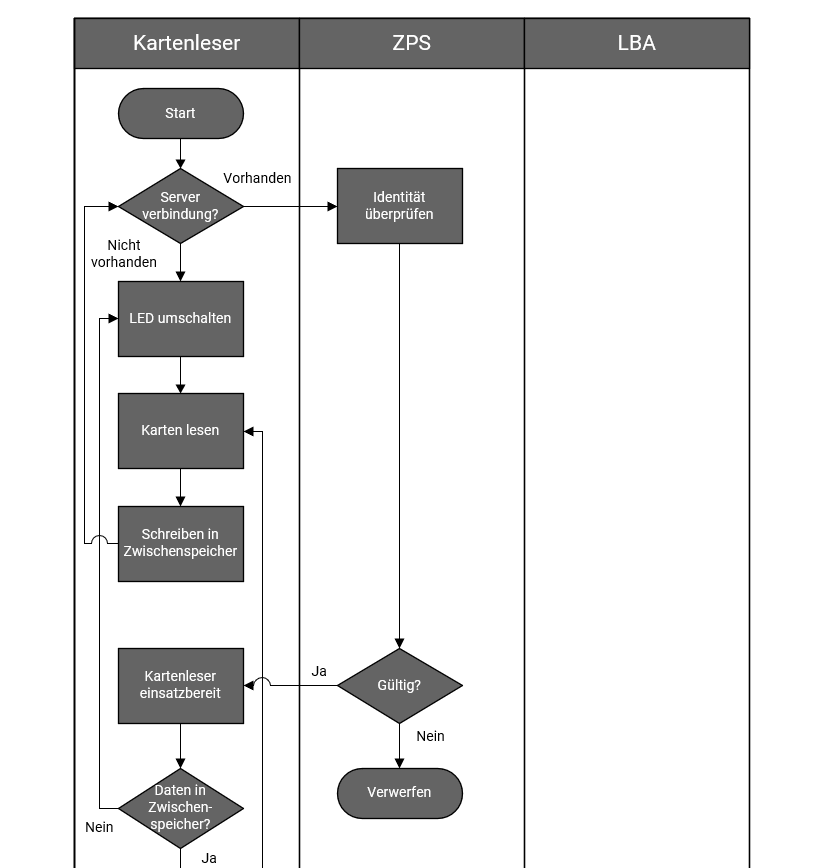
\includegraphics[width=\textwidth]{images/visio1.png}
\newpage
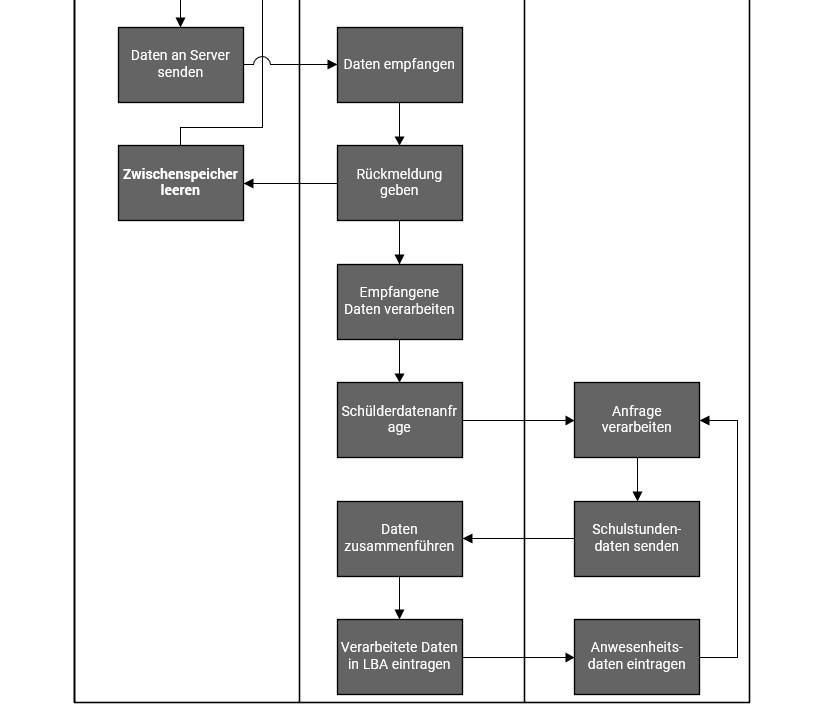
\includegraphics[width=\textwidth]{images/visio2.png}

\section{Technische Machbarkeit}
\subsection{Technologien}
Das Gesamtpaket des \gls{lbvt} besteht aus den Kartenlesegeräten, dem \gls{zps} und der \gls{lba}-Schnittstelle der Schule
\subsubsection{Kartenleser}
Auf den Kartenlesegeräten läuft eine lokale Datenbank und Software, welche in der Lage ist Kartendaten zu lesen, diese in die Datenbank zwischenzuspeichern und anschließend an den \gls{zps} weiterzuleiten. Die Programmiersprache der Software wird durch den Hardware Support festgelegt und ist vergleichsweise irrelevant. Die Datenbank muss performant und ressourcensparend arbeiten, da eine begrenzte Akkukapazität vorhanden ist.
\subsubsection{ZPS}
Der \gls{zps} wird auf einem Server im Schulnetzwerk untergebracht. Aus kompatiblitätsgründen kommt nur die Linux-Distribution Ubuntu als Serverbetriebssystem in Frage. Weiters muss auf dem \gls{zps} ein Webinterface zur Datenausgabe bereitgestellt werden. Die Programmiersprache der Software ist auch hier relativ irrelevant, da die Netzwerkprotokolle unabhängig davon arbeiten können.
\subsection{Variantenbildung}
Für die wichtigsten Kerntechnologien des \gls{lbvt} werden nachfolgende bestehende Lösungsvarianten ausgewählt und mit Hilfe einer Nutzwertanalyse bewertet, um die optimale Lösungsvariante zu erhalten. Jede Unterkategorie der Nutzwertanalyse wird mit Punkten von 0 bis 100 bewertet und anschließend mit der Gewichtung multipliziert. Die Summe aus diesen Werten ist dann der Gesamtwert einer Variante.
\subsubsection{Kartenleser - Hardware}
Es gibt viele Möglichkeiten um Eingebettete Systeme zu entwickeln, jedoch bieten sich für den Einsatz als Kartenlesegerät hauptsächlich zwei Architekturen, welche für den Einsatz realistisch wären. Einerseits die Raspberry Pi Architektur, welche auf Linux aufsetzt und wie ein PC verwendbar ist, andererseits ist es möglich einen Mikrocontroller von STMicroelectronics einzusetzen.
\vspace{0.2cm}\\
Die Kriterien für die Nutzwertanalyse bestehen aus der Dokumentation, Kompatibilität, Sicherheit, Energieverbrauch und der Erfahrung des Projektteams, mit diesen Architekturen umzugehen. Hierbei liegt das Hauptaugenmerk auf der Dokumentation und der Kompatibilität welche jeweils mit 30\% gewichtet werden. Die Dokumentation des Systemaufbaus, der Hilfestellungen und Bibiliotheken sind wichtig um eine effiziente Realisierung zu ermöglichen. Die Kompatibilität der Architekturen ist etwas schwieriger zu Quantisieren, jedoch fallen in diese Kategorie das vorhandene Software-Angebot und die Kompatibilität mit bestehenden Technologien im Schulsystem.\vspace{0.2cm}\\
Die Sicherheit der Implementierung ist der nächst wichtige Punkt und wird mit 20\% bewertet. Da die Geräte heikle Daten wie Anwesenheit verarbeiten, wäre eine Kompromittierung der Systeme verheerend. Der Energieverbrauch der Systeme wirkt sich auf die Nutzungsdauer aus, welche im Idealfall endlos wäre. Da die Vorgaben des Auftraggebers berücksichtigt werden müssen, wird dieser Punkt mit 10\% bewertet. Der letzte Punkt umfasst die Geübtheit der Teammitglieder mit den Architekturen umzugehen. Es ist wichtig, dass das Projektteam bereits Erfahrung besitzt um Fehler vorzubeugen und die Effizienz der Entwicklung zu steigern. Daher wird auch dieser Aspekt mit 10\% bewertet.\vspace{0.2cm}\\ Die Kosten fallen nicht in die Analyse, da beide Geräte sich im Preis um unter 1\% unterscheiden.\\
\begin{tabular}{| p{2.2cm} |  p{2.2cm} | p{1.4cm} |  p{1.4cm} | p{1.4cm} | p{1.4cm} | p{1.4cm} | }
        \cline{3-7}
        \multicolumn{2}{c|}{} &  \cellcolor{gray} & \multicolumn{2}{|c|}{\cellcolor{gray} \color{white}Raspberry} & \multicolumn{2}{|c|}{\cellcolor{gray} \color{white}STM32}  \\
        \cline{4-7} 
        \multicolumn{2}{c|}{} &  \cellcolor{gray} & Punkte & \multirow{2}{*}{\parbox{1.4}{\footnotesize \mbox{Punkte mit} Gewich-tung}} & Punkte & \multirow{2}{*}{\parbox{1.4}{\footnotesize \mbox{Punkte mit} Gewich-tung}}   \\ 
        %\multicolumn{2}{c|}{} & & & & &  \\
        \multicolumn{2}{c|}{} &  \cellcolor{gray}\multirow{-3}{*}{\parbox{1.4cm}{\color{white}Gewich-tung in \%}} & & & &  \\
        \hline
        \cellcolor{gray}\color{white}Doku&\cellcolor{lightgray}\color{white}Umfang & 15 & 100 & 15 & 80 & 12 \\
        \cline{2 -7}
        \cellcolor{gray} &\cellcolor{lightgray}\color{white}Struktur & 5 & 80 & 4 & 40 & 2 \\
        \cline{2 -7}
        \cellcolor{gray} &\cellcolor{lightgray}\color{white}API Beschreibung & 10 & 70 & 7 & 20 & 2\\
        \cline{2 -7}
        \cellcolor{gray} &\cellcolor{lightgray}\color{white}Gesamt & \cellcolor{lightgray}\color{white}30 & \cellcolor{lightgray}\color{white}250 & \cellcolor{lightgray}\color{white}26 & \cellcolor{lightgray}\color{white}140 & \cellcolor{lightgray}\color{white}16\\
        \cline{2 -7}
        \cellcolor{gray}\color{white}Kompatibilität&\cellcolor{lightgray}\color{white}Softwarean- gebot & 15 & 90 & 13.5 & 70 & 10.5 \\
        \cline{2 -7}
        \cellcolor{gray} &\cellcolor{lightgray}\color{white}Schulsystem & 15 & 90 & 13.5 & 70 & 10.5 \\
        \cline{2 -7}
        \cellcolor{gray} &\cellcolor{lightgray}\color{white}Gesamt & \cellcolor{lightgray}\color{white}30 & \cellcolor{lightgray}\color{white}180 & \cellcolor{lightgray}\color{white}27 & \cellcolor{lightgray}\color{white}140 & \cellcolor{lightgray}\color{white}21\\
        \cline{2 -7}
        \cellcolor{gray}\color{white}Sicherheit&\cellcolor{lightgray}\color{white}Zertifikate & 10 & 100 & 10 & 0 & 0 \\
        \cline{2 -7}
        \cellcolor{gray} &\cellcolor{lightgray}\color{white}\small Zugriffsschutz & 10 & 40 & 4 & 100 & 10 \\
        \cline{2 -7}
        \cellcolor{gray} &\cellcolor{lightgray}\color{white}Gesamt & \cellcolor{lightgray}\color{white}20 & \cellcolor{lightgray}\color{white}140 & \cellcolor{lightgray}\color{white}14 & \cellcolor{lightgray}\color{white}100 & \cellcolor{lightgray}\color{white}10\\
        \cline{2 -7}
        \cellcolor{gray}\color{white}Energiever- brauch&\cellcolor{lightgray}\color{white}Energiever- brauch & 10 & 50 & 5 & 100 & 10 \\
        \cline{2 -7}
        \cellcolor{gray} &\cellcolor{lightgray}\color{white}Gesamt & \cellcolor{lightgray}\color{white}10 & \cellcolor{lightgray}\color{white}50 & \cellcolor{lightgray}\color{white}5 & \cellcolor{lightgray}\color{white}100 & \cellcolor{lightgray}\color{white}10\\
        \cline{2 -7}
        \cellcolor{gray}\color{white}Erfahrung&\cellcolor{lightgray}\color{white}Erfahrung & 10 & 70 & 7 & 20 & 2 \\
        \cline{2 -7}
        \cellcolor{gray} &\cellcolor{lightgray}\color{white}Gesamt & \cellcolor{lightgray}\color{white}10 & \cellcolor{lightgray}\color{white}70 & \cellcolor{lightgray}\color{white}7 & \cellcolor{lightgray}\color{white}20 & \cellcolor{lightgray}\color{white}2\\
        \cline{2 -7}
        \multicolumn{2}{|c|}{\cellcolor{gray}\color{white}Gesamtwertung} & 100 & \multicolumn{2}{|r|}{79} & \multicolumn{2}{|r|}{59}\\
        \hline
    \end{tabular} 

\subsubsection{Kartenleser - Datenbank}
Es gibt mehrere gängige Datenbanksysteme, jedoch sind die meisten nicht dafür geeignet auf einem eingebetteten System zu laufen. Daher kommen nur Systeme in Frage, welche darauf ausgelegt sind, auf solchen Systemen zu arbeiten. Hier werden die Datenbanksysteme SQLite und SQLCipher verglichen.\vspace{0.2cm}\\
Die Kriterien der Nutzwertanalyse bestehen aus der Sicherheit mit 30\%, da sensible Daten gespeichert werden können, so wie die Effizienz mit 40\% Gewichtung. In letzteres fallen beispielsweise der Verbrauch von Ressourcen und Zugriffsgeschwindigkeit auf Daten. Letztendlich wird noch die Kompatibilität und Kosten mit jeweils 15\% gewichtet. Die Kompatibilität bezieht sich hierbei auf vorhandenen Code und die Plattform auf der die Datenbank laufen wird.\\
\begin{tabular}{| p{2.2cm} |  p{2.2cm} | p{1.4cm} |  p{1.4cm} | p{1.4cm} | p{1.4cm} | p{1.4cm} | }
        \cline{3-7}
        \multicolumn{2}{c|}{} &  \cellcolor{gray} & \multicolumn{2}{|c|}{\cellcolor{gray} \color{white}SQLite} & \multicolumn{2}{|c|}{\cellcolor{gray} \color{white}SQLCipher}  \\
        \cline{4-7} 
        \multicolumn{2}{c|}{} &  \cellcolor{gray} & Punkte & \multirow{2}{*}{\parbox{1.4}{\footnotesize \mbox{Punkte mit} Gewich-tung}} & Punkte & \multirow{2}{*}{\parbox{1.4}{\footnotesize \mbox{Punkte mit} Gewich-tung}}   \\ 
        %\multicolumn{2}{c|}{} & & & & &  \\
        \multicolumn{2}{c|}{} &  \cellcolor{gray}\multirow{-3}{*}{\parbox{1.4cm}{\color{white}Gewich-tung in \%}} & & & &  \\
        \hline
        \cellcolor{gray}\color{white}Sicherheit&\cellcolor{lightgray}\color{white}Verschlüsse- lung & 25 & 0 & 0 & 100 & 25 \\
        \cline{2 -7}
        \cellcolor{gray} &\cellcolor{lightgray}\color{white}Zugriffsge- schwindigkeit & 5 & 0 & 0 & 80 & 4 \\
        \cline{2 -7}
        \cellcolor{gray} &\cellcolor{lightgray}\color{white}Gesamt & \cellcolor{lightgray}\color{white}30 & \cellcolor{lightgray}\color{white}0 & \cellcolor{lightgray}\color{white}0 & \cellcolor{lightgray}\color{white}180 & \cellcolor{lightgray}\color{white}29\\
        \cline{2 -7}
        \cellcolor{gray}\color{white}Effizienz&\cellcolor{lightgray}\color{white}Ressourcen- verbrauch & 30 & 80 & 24 & 70 & 21 \\
        \cline{2 -7}
        \cellcolor{gray} &\cellcolor{lightgray}\color{white}Zugrifsge- schwindigkeit & 10 & 90 & 9 & 90 & 9 \\
        \cline{2 -7}
        \cellcolor{gray} &\cellcolor{lightgray}\color{white}Gesamt & \cellcolor{lightgray}\color{white}40 & \cellcolor{lightgray}\color{white}170 & \cellcolor{lightgray}\color{white}33 & \cellcolor{lightgray}\color{white}160 & \cellcolor{lightgray}\color{white}30\\
        \cline{2 -7}
        \cellcolor{gray}\color{white}Kompatibilität&\cellcolor{lightgray}\color{white}Plattform & 7.5 & 100 & 7.5 & 100 & 7.5 \\
        \cline{2 -7}
        \cellcolor{gray} &\cellcolor{lightgray}\color{white}Code & 7.5 & 100 & 7.5 & 70 & 5.25 \\
        \cline{2 -7}
        \cellcolor{gray} &\cellcolor{lightgray}\color{white}Gesamt & \cellcolor{lightgray}\color{white}15 & \cellcolor{lightgray}\color{white}200 & \cellcolor{lightgray}\color{white}15 & \cellcolor{lightgray}\color{white}170 & \cellcolor{lightgray}\color{white}12.75\\
        \cline{2 -7}
        \cellcolor{gray}\color{white}Kosten&\cellcolor{lightgray}\color{white}Kosten & 15 & 100 & 15 & 100 & 15 \\
        \cline{2 -7}
        \cellcolor{gray} &\cellcolor{lightgray}\color{white}Gesamt & \cellcolor{lightgray}\color{white}15 & \cellcolor{lightgray}\color{white}100 & \cellcolor{lightgray}\color{white}15 & \cellcolor{lightgray}\color{white}100 & \cellcolor{lightgray}\color{white}15\\
        \cline{2 -7}
        \multicolumn{2}{|c|}{\cellcolor{gray}\color{white}Gesamtwertung} & 100 & \multicolumn{2}{|r|}{63} & \multicolumn{2}{|r|}{86.75}\\
        \hline
    \end{tabular}

\subsection{Umsetzbarkeit}
Die Machbarkeit des \gls{lbvt} ist aus technischer Sicht gewährleistet, da die benötigten Technologien vorhanden sind und für die Umsetzung geeignet sind.
\section{Wirtschaftliche Machbarkeit}
\subsection{Aufwandschätzung}
Der Aufwand für das Projekt, also die Projektkoste, ergeben sich aus dem Personalaufand und dem Investitionsaufwand.
\subsubsection{Personalaufwand}
Der Personalaufwand beschreibt die voraussichtlichen Kosten des Projektteams und wird aus den erwarteten Stunden und dem Stundensatz berechnet.\\
\begin{center}
    \begin{tabular}{| l | l | l | l |}
        \hline \rowcolor{gray} \textbf{\textcolor{white}{Person}} & \textbf{\textcolor{white}{Stunden}} & \textbf{\textcolor{white}{Stundensatz in €}}& \textbf{\textcolor{white}{Kosten in €}}\\
        \hline
        Manuel Kisser& 60 & 75 & 4500\\
        \hline
        Kacper Urbaniec& 60 & 80 & 4800\\
        \hline
        Moritz Welsch& 60 & 75 & 4500\\
        \hline
        Martin Wustinger& 60 & 75 & 4500\\
        \hline
    \end{tabular}
\end{center}
\subsubsection{Investitionsaufwand}
Das \gls{lbvt} benötigt Kartenlesehardware und einen Ubuntu-Server für den \gls{zps}. Da beide System freie Software und Betriebssysteme verwenden fallen keine laufenden Lizenzkosten an. Letzendlich muss für die Replikation der Kartenlesegeräte ein Techniker 1-2 Stunden pro Gerät aufwenden, um diese zusammen zu bauen, in das System einzubinden und letztendlich um diese zu testen. Letztendlich fallen laufende Kosten für die Wartung an. Es müssen Kosten für Strom und Internet für das System gedeckt werden. Der Mikrocontroller vom Kartenleser besitzt eine durchschnittliche Lebenspanne von zehn bis fünfzehn Jahren, kann aber bei guter Wartung länger im Betrieb bleiben. Nach zehn Jahren sollte man aber schon nachdenken, ob es sich lohnt auf neuere Modelle umzusteigen, welche vielleicht niedrigere Stromkosten bieten. Falls die Kartenleser Speicher in der Form von Flash (SD-Karten, etc.) besitzen, muss man davon ausgehen, dass sie innerhalbe der Lebenspanne des Kartenlesers mindestens einmal ausgetauscht werden müssen.
\subsection{Nutzen}
Es sind keine direkten Projekteinnahmen zu erwarten, falls zukünftig Klassenbücher komplett durch das Lernbüroverwaltungssystem ersetzt werden, kann pro Jahr circa 6 € pro Klasse nur an reinem Papier Geld gespart werden. Außerdem müssen Klassenvorstände nicht mehr für eine Stunde pro Woche bezahlt werden, in der sie die Klassenbücher manuell in das System eintragen.
\subsection{Risikoanalyse}
\begingroup
\renewcommand*{\arraystretch}{1.1} % Abstand zwischen Zeilen
\begin{center}
\begin{tiny}
\begin{tabularx}{\textwidth}{|l|p{1.1cm}|X|l|l|l|p{0.5cm}|l|X|l|}
    \hline
    \multicolumn{10}{|c|}{\vspace{-0.02cm} \rowcolor{gray}} \\
    \multicolumn{10}{|c|}{\rowcolor{gray} \bfseries \normalsize \color{white} PROJEKTRISIKOANALYSE \vspace{-0.05cm}} \\
    \multicolumn{10}{|c|}{\rowcolor{gray}} \\
    \hline
    & & & & & & & & &\\
    & & Risiko- & & & Eintritts- & & & Präventive & Risiko-\\
    PSP- & Arbeitspaket- & beschreibung, & & Risiko- & wahrschein- & Risiko- & Ver- & korrektive & minimierungs- \\
    Code & bezeichnung & Ursache & Priorität & kosten & lichkeit & wert & zögerung & Maßnahmen & kosten \\
    \hline 
    (Code) & (Text) & (Text) & (Auswahl) & (Euro) & (Prozent) & (Euro) & (Wochen) & (Text) & (Euro) \\
    \hline
    [0303] & Einbau der Serv.-Software in Netzwerk & Schwierig- keiten beim Aufsetzen des Serversystems im Schulnetzwerk & 2 & €750 & 10\% & & 1 & Abstimmung mit IT-Service über vorhandene Netzwerkstruktur und Anweisungen um einen Server im Schulnetzwerk aufzusetzen &-\\
    \hline
    [0305]& Verbindung von Cardreader und Server & Netzwerkrout- ing-Probleme im Schulnetzwerk & 1 & €1200+ & 5\% & & 3+ & Absprache mit IT-Service über Netzwerk & -\\
    \hline
    [0305]& Verbindung von Cardreader und Server & Kommunika- tionsprobleme zwischen Cardreader und Server & 1 & €1200+ & 40\% & & 3+ & Absprache mit IT-Service über Netzwerk & -\\
    \hline
    [0301]& Cardreader-Software & Probleme beim Lesen von Kartendaten & 2 & €250 & 15\% & & <1 & Vergleich mit existierender Kartenleser Technologie, Absprache mit Kartenhersteller & €50\\
    \hline
    [0302]& Server-Software & Probleme bei der Zuordnung von Kartendaten zu Schulstunden & 2 & €750 & 30\% & & 2 & Absprache mit IT-Service und LDAP Betreiber & -\\
    \hline
    [0302]& Server-Software & Probleme bei der Übersetzung von Kartendaten zu Schüler-ID & 2 & €750 & 30\% & & 2 & Absprache mit IT-Service und LDAP Betreiber & -\\
    \hline
    & & Projektteilziele harmonisieren nicht miteinander & 3 & €350 & 5\% & & 1-2 & Vorausplanung mit Hilfe von Lehrern & -\\
    \hline
    & & Krankheitsbe- dingter Ausfall eines Teammitglieds & 2 & €900 & 80\% & & 2 & Gesundheits- zustand der Teammitglieder in Planungszeit einberechnen & -\\
    \hline
    & & Projektbudget wird nicht zur Verfügung gestellt & 1 & €150 & 95\% & & 0 & Quasi unausweichlich da Mittel der Schule durch Steuerskandal eingefroren wurden & €150\\
    \hline
    \multicolumn{2}{|l|}{Summe Projekt} & & & €6300 & & & 15+ & &€200\\
    \hline
\end{tabularx}
\end{tiny}
\end{center}
\endgroup
\begin{flushleft}
Die Priorität wird von eins an aufsteigend bewertet, wobei 1. die höchste Priorität besitzt.
\end{flushleft}
\newpage

\section{Persönliche Machbarkeit}
Die Umsetbarkeit des \gls{lbvt} ist durch die Erfahrung aller Projektteammitglieder gegeben. Herr Kisser und Herr Urbaniec haben beim Programmieren von Robotern bereits etwas Know-How in Bezug auf proprietäre Mikrocontroller gesammelt. Das gesamte Projektteam hat in der Ausbildung sowohl mit Microcontrollern als auch mit den Programmiersprachen C, Python und Java bereits gearbeitet. Außerdem hat das Projektteam auch schon Projekte in Bezug auf REST-Schnittstellen abgeschlossen, deren Wissen sich sicher positiv auf die Projektentwicklung auswirken wird. Herr Kisser wird sich hauptsächlich um den Kartenleser kümmern, wobei Herr Welsch und Herr Wustinger sich eher um den \gls{zps} bzw. die Grafische Oberfläche kümmern werden. Die Hauptaufgabe vom Herrn Urbaniec wird das Projektcontrolling sein, wobei sich viele Aufgabenbereiche überschneiden werden.
\section{Projektorganisation}
Das Projektteam besteht aus dem Projektleiter Herr Kacper Urbaniec, dem Hardwareverantwortlichen Herr Manuel Kisser und den Programmierern Herr Moritz Welsch und Herr Martin Wustinger. Der direkte Ansprechpartner und Auftraggeber des Projekts ist Herr Christoph Roschger. Ein weiterer Ansprechpartner ist Herr Dominik Fürnsin der Leiter des IT-Service am TGM, welcher die benötigte Infrastruktur bereitstellt.\\
\begin{center}
    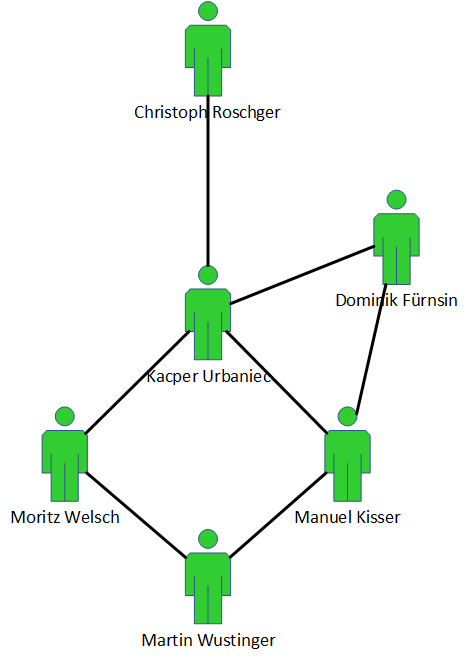
\includegraphics[width=6.9cm]{images/Projektorganisation.png}
\end{center}

\section{Projekplanung}
\subsection{Projektstrukturplan}
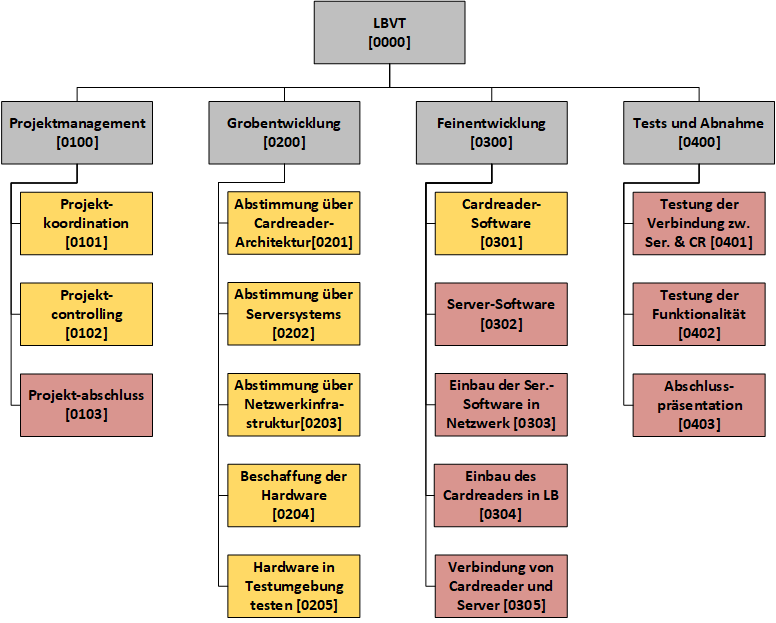
\includegraphics[width=\textwidth]{images/PSP.png}

\newpage
\subsection{Meilensteinplan}
Der Meilensteinplan beschreibt die Meilensteine, die Teilergebnisse des Projektes, zusammen mit den dazugehörigen Terminen. Diese Termine können sich im Verlauf des Projektes verschieben und geben daher nur einen gröberen Einblick auf den Zeitplan. Die Einhaltung des Start- und Endtermines hat aber hohe Priorität für das Projektteam. Außerdem liefert der Meilensteinplan Deliverables, die Liefergegenstände, die erbracht werden sollen, um einen Meilenstein abschließen zu können. 
\begin{footnotesize}
\begin{center}
    \rowcolors{2}{white}{lightgrey}
    \begin{tabularx}{\textwidth}{| p{4cm} | p{7.5cm} | X |}
        \hline \rowcolor{gray} \textbf{\textcolor{white}{Meilenstein}} & \textbf{\textcolor{white}{Deliverable}} & \textbf{\textcolor{white}{Termin}}\\
        \hline \hline
        Start & Alle benötigten Dokumente und Hefte & 21.09.2018 \\
        \hline
        Abstimmung bezüglich Kartenleserarchitektur, dem vorhandenen Serversystem und der Netzinfrastruktur & Protokolle der unterschiedlichen Projektmeetings & 05.10.2018 \\
        \hline
        Bestimmung der \gls{lbvt} Hardware Spezifikationen und deren Bestellung & Liste mit allen benötigten Hardwarekomponenten und deren Stückzahl, Bestellbestätigung & 12.10.2018 \\
        \hline
        Hardware des \gls{lbvt} ist angekommen, zusammengebaut und erstmal in Testumgebung zum laufen gebracht worden & Testbericht der ersten Tests und fertig zusammengebaute Hardware & 20.10.2018 \\
        \hline
        Die Kartenleser-Software ist fertig ausprogrammiert und auf den Kartenleser überspielt & Ein Kartenleser welcher Karten einlesen kann und seine Ergebnisse innerhalb der Testumgebung versendet & 4.11.2018 \\
        \hline
        Der \gls{zps} ist fertig ausprogrammiert und einsatzbereit & Software des \gls{zps} & 25.11.2018 \\
        \hline
        Der \gls{zps} und der Kartenleser sind miteinander verbunden und in ihre endgültigen Umgebungen eingebaut. Ab jetzt beginnen die Tests & \gls{zps} und Kartenleser & 02.12.2018 \\
        \hline
        Ende & Schüler können sich mit ihren Schülerkarten im Schulnetzwerk anmelden & 20.12.2018 \\
        \hline
    \end{tabularx}
\end{center}
\end{footnotesize}

\newpage
\section{Management Summary}
Die IT-Abteilung der Höheren Technischen Bundeslehranstalt TGM besitzt mehrere Jahrgänge, die als Schultyp das Lernbüro besitzen. Lernbüroschüler können selbst ihren Unterricht auswählen und einteilen, um einen selbstbestimmteren Schulablauf zu ermöglichen. Die Anwesenheit dieser wird derzeit noch händisch von den Lehrkräften kontrolliert. Deshalb wurde das Projektteam gebeten, diesen Prozess zu vereinfachen und informationstechnisch umzusetzen. 
\vspace{0.2cm} \\
Die Umsetzung erfolgt per Kartenleser, dazugehörigen \gls{zps} und der Integration des Projektes in die \gls{lba}. Zu erwähnen ist noch, dass das Projetteam beauftrage wurde, nur einen Kartenleser als Muster anfertigen zu lassen, der sich aber mit minimalen Aufwand nachbauen lassen kann.
\vspace{0.2cm} \\
Die Anforderungen an das \gls{lba} sind daher das Einlesen von Schülerkarten an einem Kartenlesern, die im Hintergrund sich abspielende Verarbeitung der Daten und das Anzeigen der Anwesenheit in der \gls{lba}. Außerdem soll ein Webservice am \gls{zps} realisiert werden, mit dem Kartenleser per Website konfiguriert werden können. 
\vspace{0.2cm} \\
Die Personalkosten des \gls{lbvt} werden auf 18 300 € geschätzt. Für Entwicklungsrechner werden Kosten  von 5000 € gerechnet. Für die Realisierung des \gls{zps} wird ein Server benötigt, von dem die Hardware auf 1 500 € geschätzt wird. Voraussichtlich wird die Erstellung eines Kartenleser-Musters 75 € kosten. 
\vspace{0.2cm} \\
Die Projektdauer wird auf drei Monate geschätzt. Als Starttermin wird der 21.09.2018 gehandelt, das Projektende wird für den 20.12.2018 erwartet.
\vspace{0.2cm} \\
Als Kleincomputer, der als Kartenleser fungieren soll, wird ein Raspberry Pi empfohlen. Mit diesen konnte schon das Projektteam Erfahrungen sammeln und ist daher mit der Raspberry-Plattform vertraut. Außerdem bietet diese eine sehr gute, im Bezug auf Umfang und Verständlichkeit, Dokumentation. Für die Realisierung der Datenbank wird SQLCipher verwendet, da es Verschlüsselungsverfahren anbieten, um die Kartenleser Daten vor Dritten schützen zu können. Als Betriebssystem für den \gls{zps} kommt nach tiefgründiger Untersuchung nur die Linux-Distribution Ubuntu in Frage, da es die nötigen Software-Kompatibilitäten besitzt. Noch dazu besitzt Ubuntu eine große Community als Wissensquelle und einen lang bewährten Kunden-Support. 
\vspace{0.2cm} \\
 Die Machbarkeit des \gls{lbvt} ist in allen Belangen erfüllt. Technisch ist das Projekt zweifellos machbar, da alle benötigten Technologien für die Erstellung des Projektes verfügbar sind. Wirtschaftlich ist ein gewisser Personalaufwand und Investitionsaufwand erforderliche, der aber einen guten finanziellen Nutzen der Firma „Flitzer“ GmbH dient. Die Persönliche Machbarkeit ist auch gegeben, da das Projektteam in allen Fachgebieten wie der Programmierung, Design und Datenbankrealisierung die erforderlichen Kenntnisse zur Umsetzung besitzt. 

\begin{comment}


\begin{center}

\begin{tabular}{|c|c|c|c|c|}

\hline
    \rowcolor{LimeGreen} \textbf{Produktqualität}&\textbf{Sehr gut}&\textbf{Gut}&\textbf{Normal}&\textbf{Irrelevant} \\
     \hline 
     Funktionalität&x&&&\\
     \hline
     Zuverlässigkeit&x&&&\\
     \hline
     Benutzbarkeit&&x&&\\
     \hline
     Effizienz&&&x&\\
     \hline
     Änderbarkeit&&x&&\\
     \hline
     Übertragbarkeit&x&&&\\
\hline
\end{tabular}
\end{center}


%LEGACY TABLE DESIGN
    \begin{tabular}{| p{2.2cm} |  p{2.2cm} | p{1.4cm} |  p{1.4cm} | p{1.4cm} | p{1.4cm} | p{1.4cm} | }
        \cline{3-7}
        \multicolumn{2}{c|}{} &  \multirow{3}{Gewich-tung in \%} & \multicolumn{2}{|c|}{\cellcolor{LimeGreen} test1} & \multicolumn{2}{|c|}{\cellcolor{LimeGreen} test2}  \\
        \cline{4-7} 
        \multicolumn{2}{c|}{} &  & Punkte & \multirow{2}{\footnotesize \mbox{Punkte mit} Gewich-tung} & Punkte & \multirow{2}{\footnotesize \mbox{Punkte mit} Gewich-tung}   \\ 
        \multicolumn{2}{c}{} & & & & & & \\
        \hline
        1 & 2 & 3 & 4 & 5 & 6 & 7 \\
        \cline{2 -7}
        1 & 2 & 3 & 4 & 5 & 6 & 7 \\
        \cline{2 -7}
        1 & 2 & 3 & 4 & 5 & 6 & 7
        
        \begin{comment}
        
        
         \multicolumn{2}{c} & & Punkte & \multirow{2}{\footnotesize \mbox{Punkte mit} Gewich-tung} & Punkte & \multirow{2}{\footnotesize \mbox{Punkte mit} Gewich-tung}   \\
         \multicolumn{2}{c} & & & & &\\
         \hline 
         1 & 2 & 3 & 4 & 5 & 6 & 7  \\
        
        \hline
        \end{comment}
     
    \end{tabular}

\end{comment}

